\documentclass[a4paper, 14pt, dvipdfmx]{extarticle}

\usepackage{animate}
\usepackage{amsmath, amssymb, amsthm, mathrsfs, amsfonts, dsfont}
\usepackage{ascmac}
\usepackage{bbm}
\usepackage{bm}
\usepackage{breakcites}
\usepackage{calc}
\usepackage[style=base]{caption}
\usepackage{enumerate}
\usepackage[T1]{fontenc}
\usepackage{ifthen}
\usepackage{mathtools}
\usepackage{makecell}
\usepackage{mlmodern}
\usepackage{newtxtext}
\usepackage{optidef}
\usepackage[deluxe]{otf}
\usepackage{physics}
\usepackage{pifont}
\usepackage{setspace}
\usepackage{stfloats}
\usepackage{subcaption}
\usepackage{svg}
\usepackage{tikz}
\usepackage{xparse}
\usepackage[all]{xy}

\usepackage{float}
\usepackage{color}
\usepackage{graphicx}
\usepackage[margin=20truemm]{geometry}
\usepackage[colorlinks=true, allcolors=blue]{hyperref}


% === Commands ===

\definecolor{cA}{HTML}{0072BD}
\definecolor{cB}{HTML}{EDB120}
\definecolor{cC}{HTML}{77AC30}
\definecolor{cD}{HTML}{D95319}
\definecolor{cE}{HTML}{7E2F8E}
\newcommand{\cAText}[1]{\textcolor{cA}{#1}}
\newcommand{\cBText}[1]{\textcolor{cB}{#1}}
\newcommand{\cCText}[1]{\textcolor{cC}{#1}}
\newcommand{\cDText}[1]{\textcolor{cD}{#1}}
\newcommand{\cEText}[1]{\textcolor{cE}{#1}}
\newcommand{\red}[1]{\textcolor{red}{#1}}
\newcommand{\blue}[1]{\textcolor{blue}{#1}}
\newcommand{\green}[1]{\textcolor{green}{#1}}
\newcommand{\gray}[1]{\textcolor{gray}{#1}}
\newcommand{\black}[1]{\textcolor{black}{#1}}

\newcommand{\st}{\text{ s.t. }}
\newcommand{\Img}[1]{\mathrm{Im}\qty(#1)}
\newcommand{\Ker}[1]{\mathrm{Ker}\qty(#1)}
\newcommand{\Supp}[1]{\mathrm{supp}\qty(#1)}
\newcommand{\Rank}[1]{\mathrm{rank}\qty(#1)}
\newcommand{\floor}[1]{\left\lfloor #1 \right\rfloor}
\newcommand{\ceil}[1]{\left\lceil #1 \right\rceil}
% C++ (https://tex.stackexchange.com/questions/4302/prettiest-way-to-typeset-c-cplusplus)
\newcommand{\Cpp}{C\nolinebreak[4]\hspace{-.05em}\raisebox{.4ex}{\relsize{-3}{\textbf{++}}}}
% https://tex.stackexchange.com/questions/28836/typesetting-the-define-equals-symbol
\newcommand{\defeq}{\coloneqq}
\newcommand{\eqdef}{\eqqcolon}
% https://tex.stackexchange.com/questions/5502/how-to-get-a-mid-binary-relation-that-grows
\newcommand{\relmiddle}[1]{\mathrel{}\middle#1\mathrel{}}
\newcommand{\cmark}{\cCText{\ding{51}}} % check mark
\newcommand{\xmark}{\red{\ding{55}}} % cross mark

\DeclareMathOperator{\Proj}{Proj}
\DeclareMathOperator{\Exp}{Exp}
\DeclareMathOperator{\Hess}{Hess}
\DeclareMathOperator{\Retr}{Retr}
\DeclareMathOperator{\Span}{span}
\DeclareMathOperator{\myGrad}{grad}
\renewcommand{\grad}{\myGrad}

% https://tex.stackexchange.com/questions/564216/newcommand-for-each-letter
\ExplSyntaxOn
\NewDocumentCommand{\definealphabet}{mmmm}{
\int_step_inline:nnn{`#3}{`#4}{
\cs_new_protected:cpx{#1 \char_generate:nn{##1}{11}}{
\exp_not:N #2{\char_generate:nn{##1}{11}}}}}
\ExplSyntaxOff

\definealphabet{bb}{\mathbb}{A}{Z}
\definealphabet{rm}{\mathrm}{A}{Z}
\definealphabet{cal}{\mathcal}{A}{Z}
% \definealphabet{scr}{\mathscr}{A}{Z}
\definealphabet{frak}{\mathfrak}{a}{z}
\definealphabet{frak}{\mathfrak}{A}{Z}

% === Settings ===

% https://qiita.com/rityo_masu/items/efd44bc8f9229e014237
\allowdisplaybreaks[4]

\usetikzlibrary{
  3d,
  fit,
  calc,
  math,
  matrix,
  patterns,
  backgrounds,
  arrows.meta,
  decorations.pathmorphing,
}

\newcommand{\IMG}[2]{
    \begin{figure}[H]
        \centering
        \includegraphics[width={#2}\columnwidth]{#1}
    \end{figure}
}

\begin{document}

\title{Supplemental Material for 10/30\\Book Reading Seminar}
\author{Hiroki Hamaguchi}
\date{\today}
\maketitle

\begin{abstract}
    \begin{center}
        This is the supplemental material for the book reading seminar.

        Please refer to the textbook and the whiteboard for the main content.

        If necessary, please also refer to the \href{https://github.com/hari64boli64/BookReadingSeminarMaterials}{repository}.
    \end{center}
\end{abstract}

\section*{3.2.1}

\begin{figure}[H]
    \begin{minipage}{0.49\columnwidth}
        \centering
        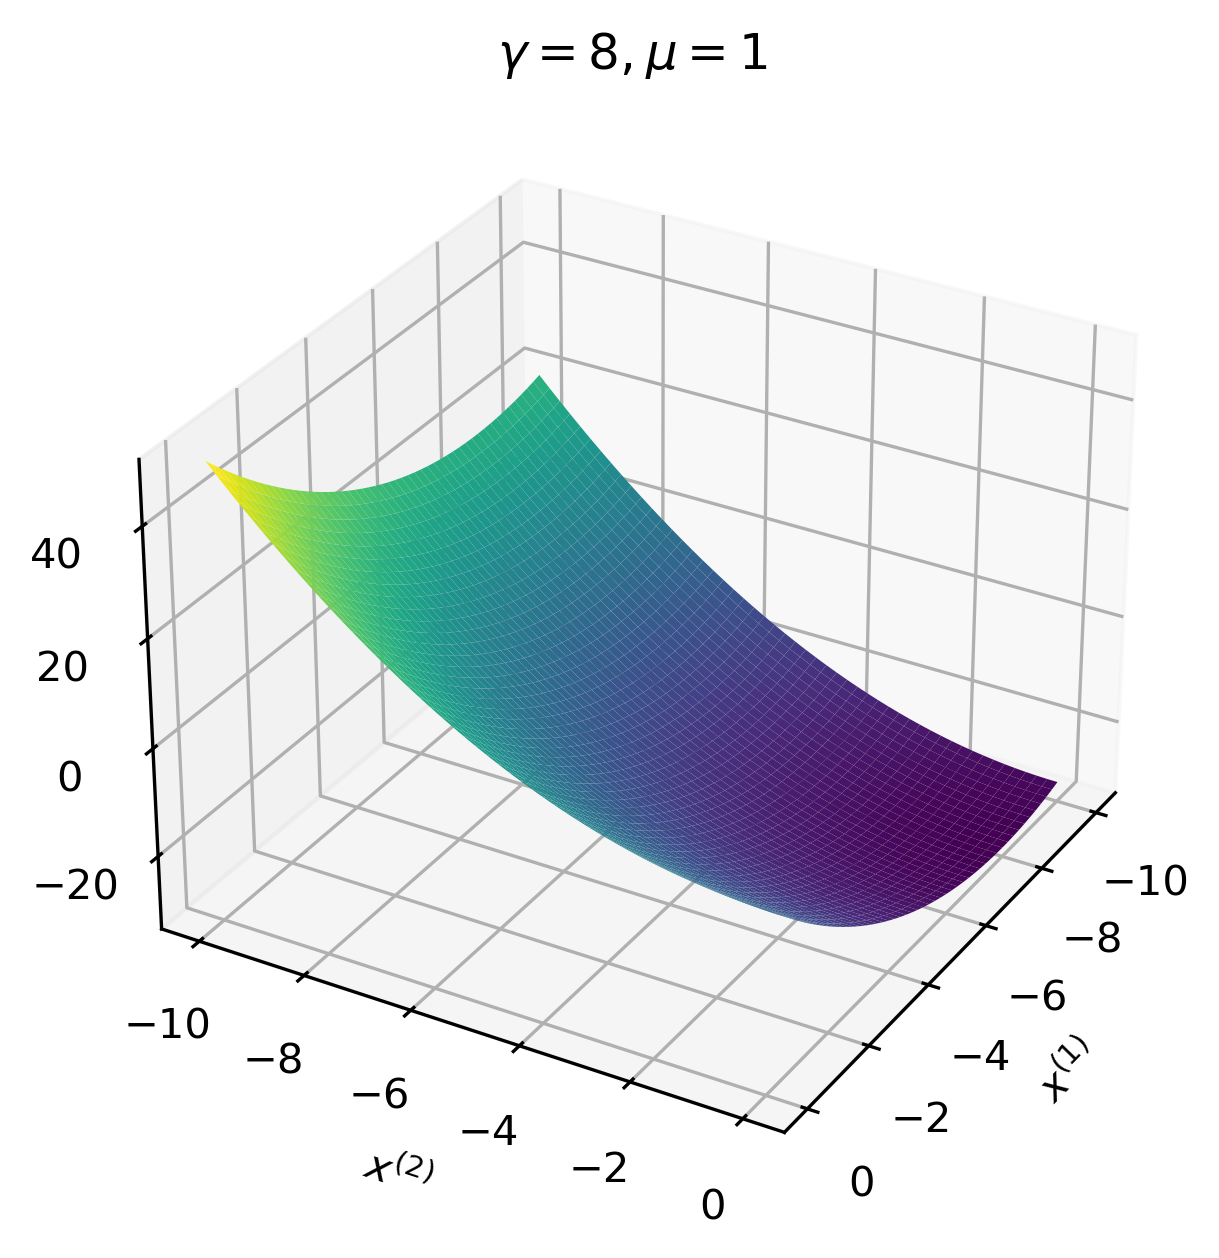
\includegraphics[width=0.6\columnwidth]{fk_1_1.png}
    \end{minipage}
    \begin{minipage}{0.49\columnwidth}
        \centering
        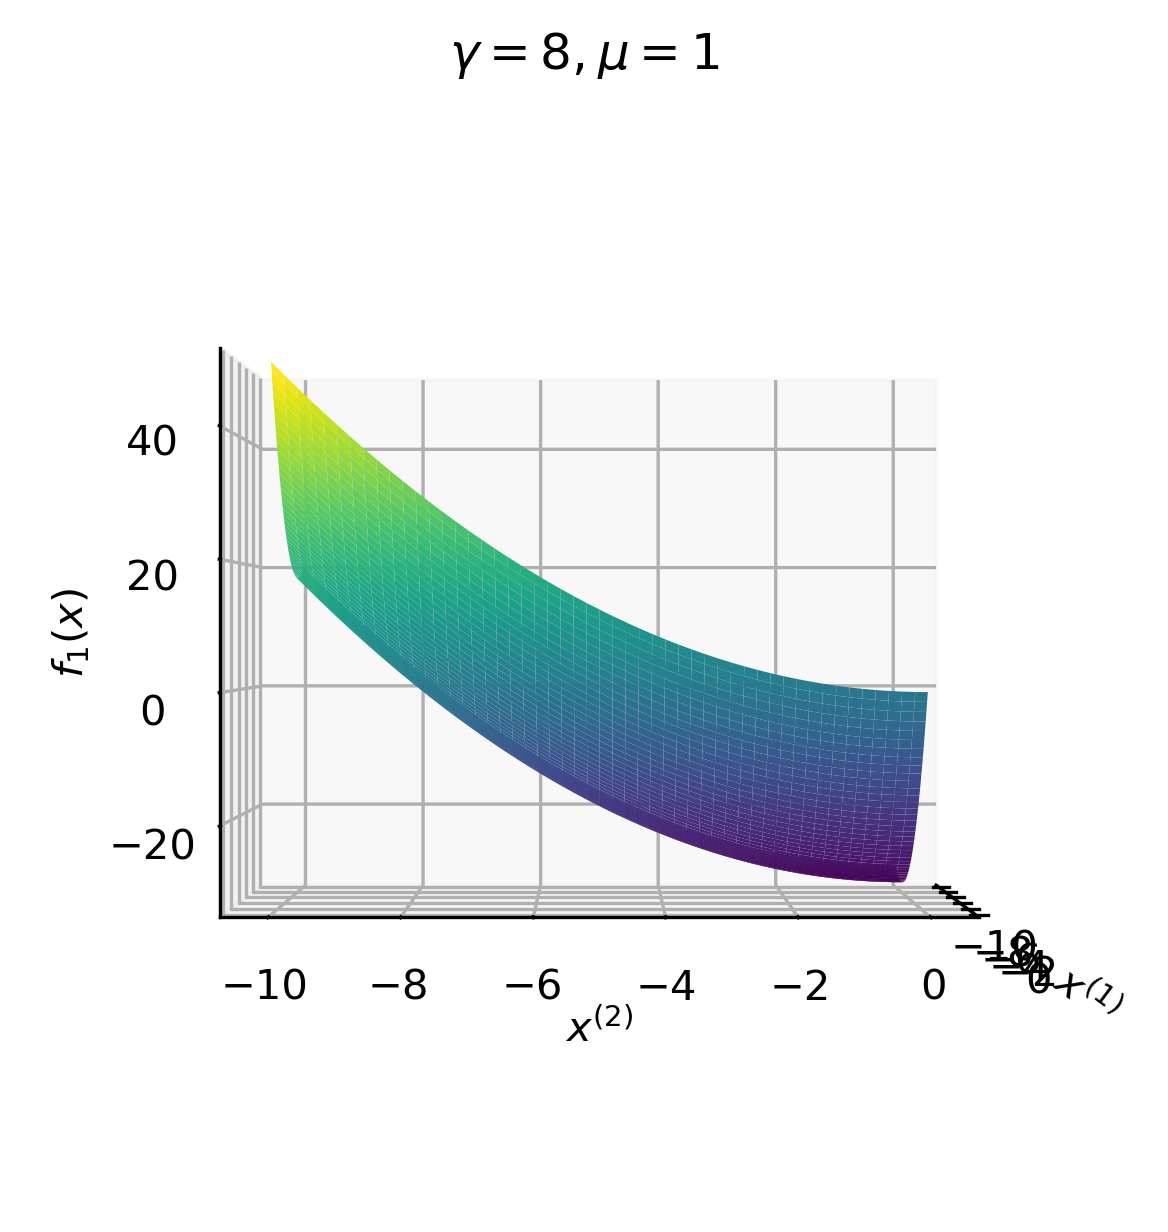
\includegraphics[width=0.6\columnwidth]{fk_1_2.png}
    \end{minipage}
\end{figure}
\begin{figure}[H]
    \begin{minipage}{0.49\columnwidth}
        \centering
        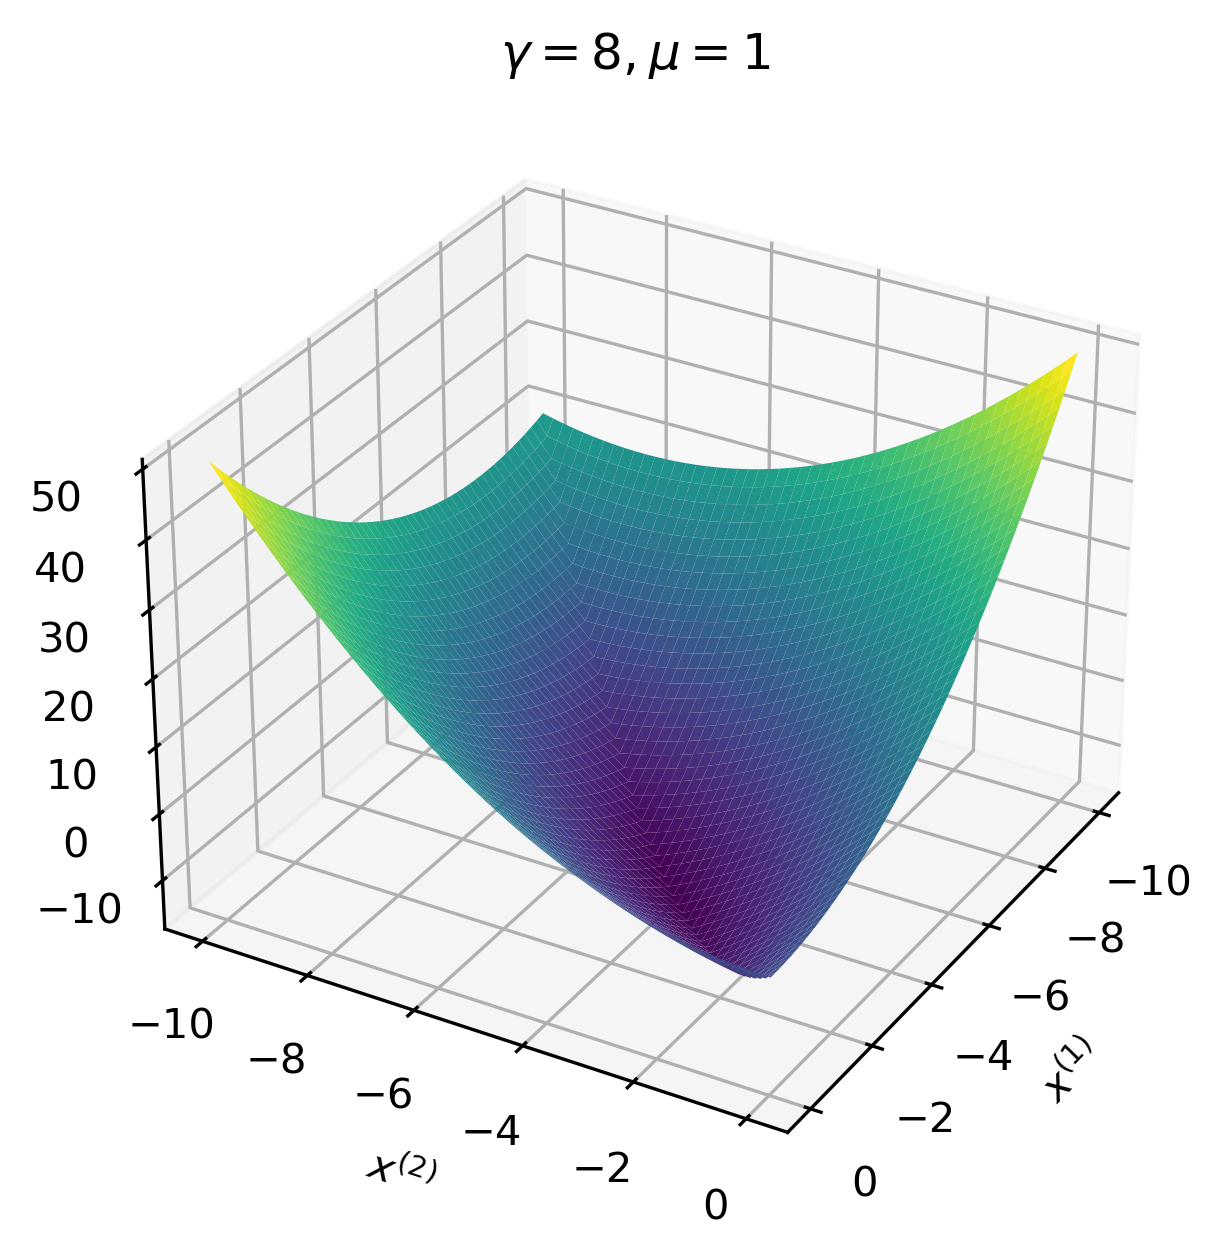
\includegraphics[width=0.6\columnwidth]{fk_2_1.png}
    \end{minipage}
    \begin{minipage}{0.49\columnwidth}
        \centering
        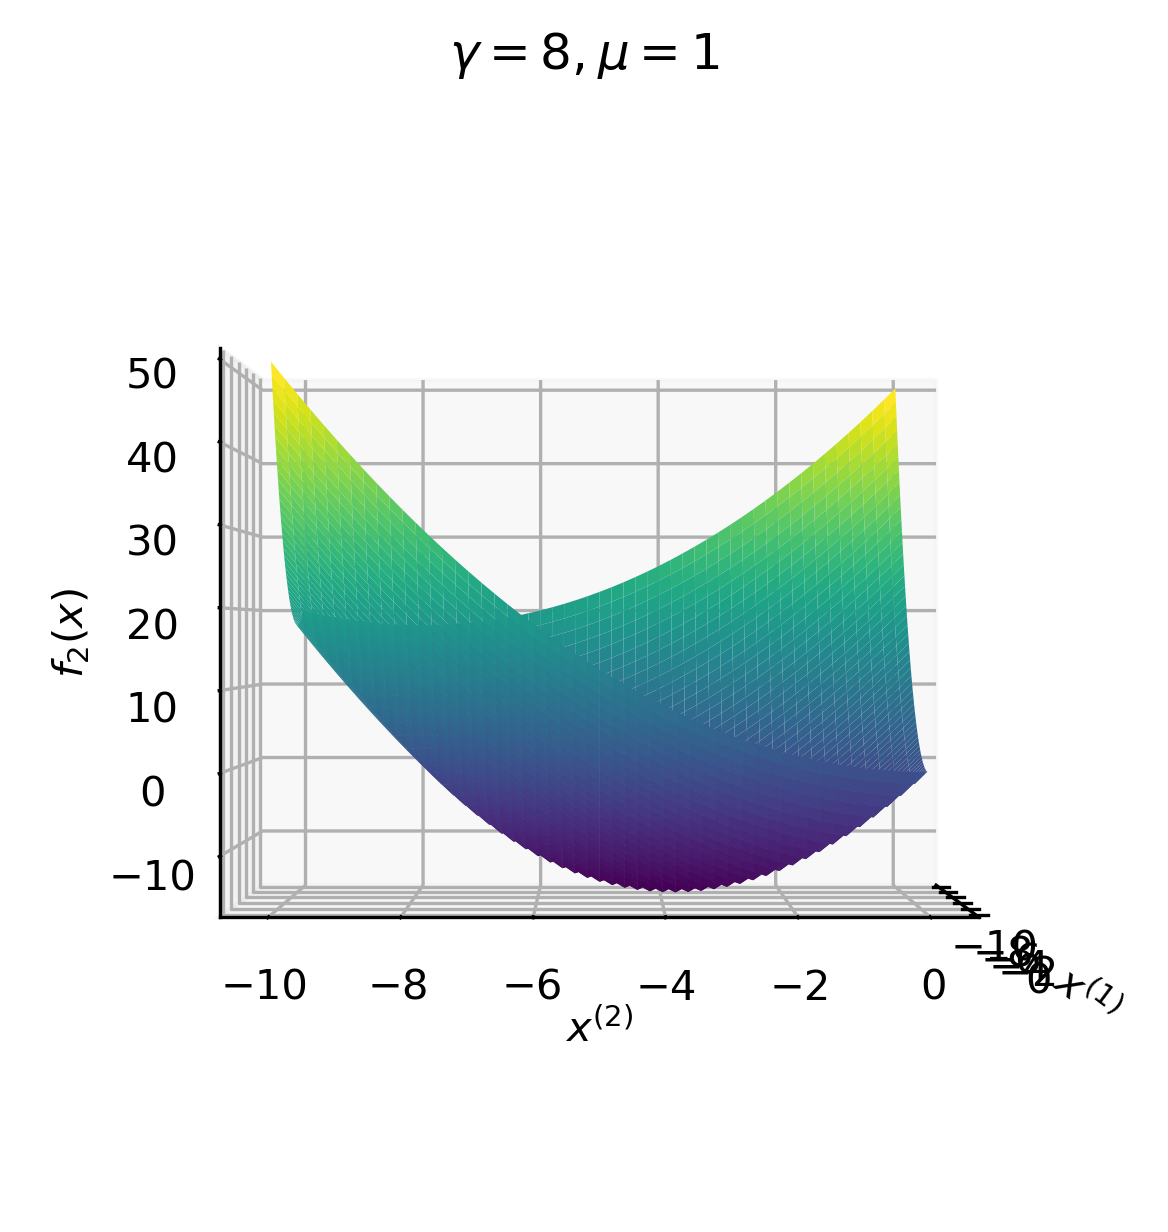
\includegraphics[width=0.6\columnwidth]{fk_2_2.png}
    \end{minipage}
\end{figure}

\begin{figure}[H]
    \centering
    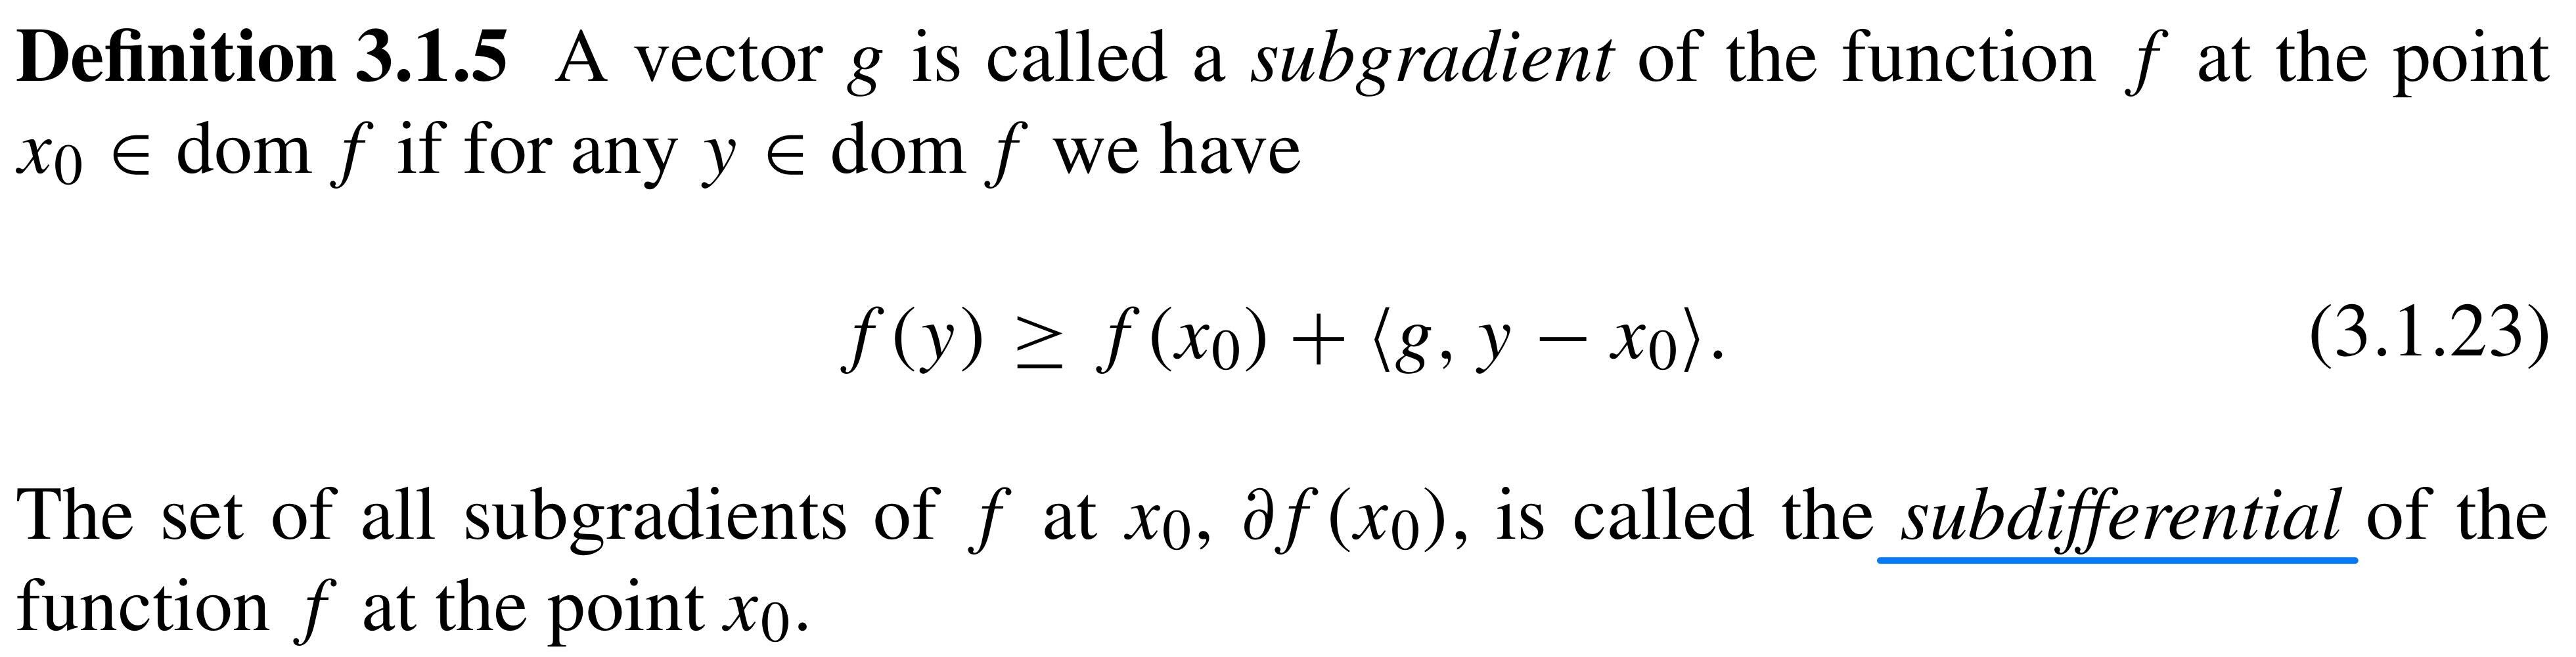
\includegraphics[width=\columnwidth]{def315.jpg}
    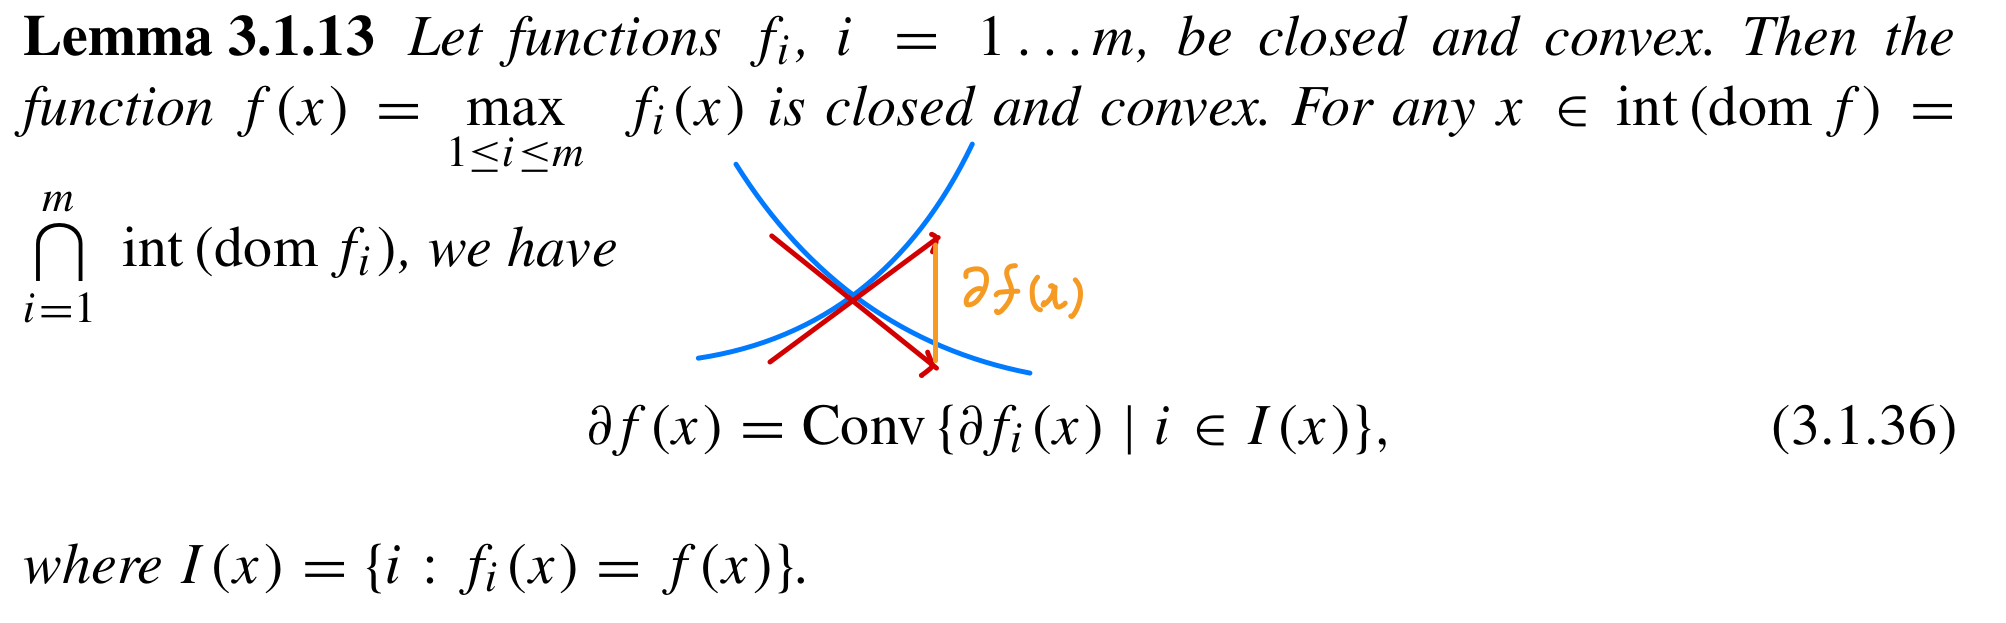
\includegraphics[width=\columnwidth]{lem3113.png}
    \caption{\red{p.195: ``described in Sect. 3.1.6''}}
\end{figure}

\begin{figure}[H]
    \centering
    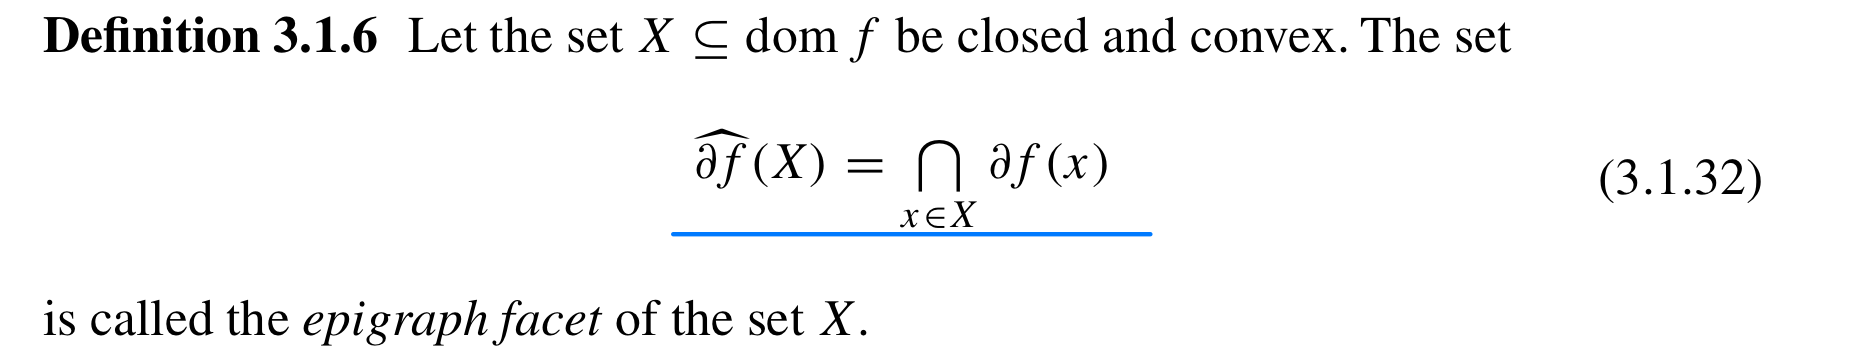
\includegraphics[width=\columnwidth]{def316.png}
    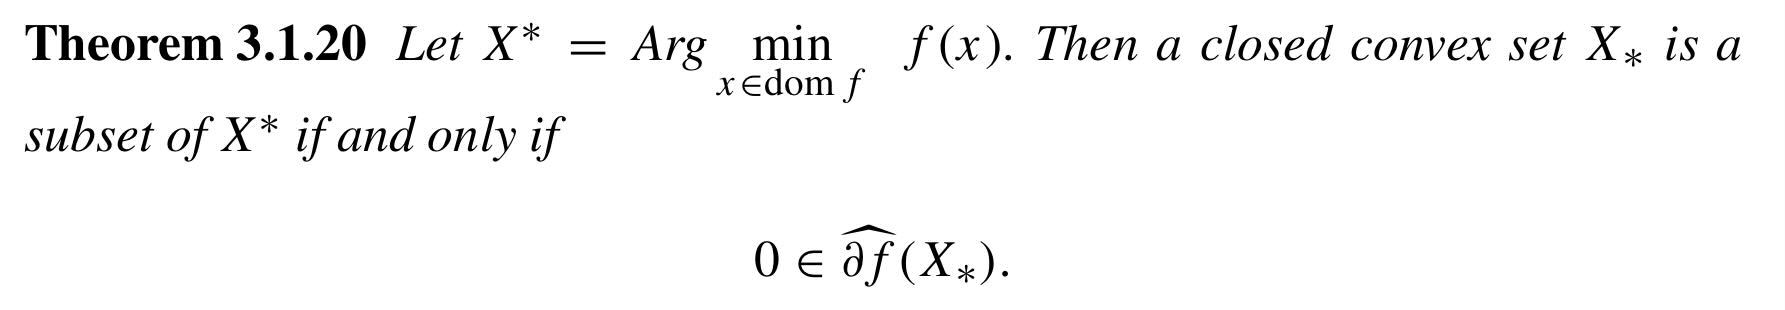
\includegraphics[width=\columnwidth]{thm3120.jpg}
    \caption{\red{p.196: ``Further, by Theorem 3.1.20,''}}
    \label{fig:label}
\end{figure}

\begin{figure}[H]
    \centering
    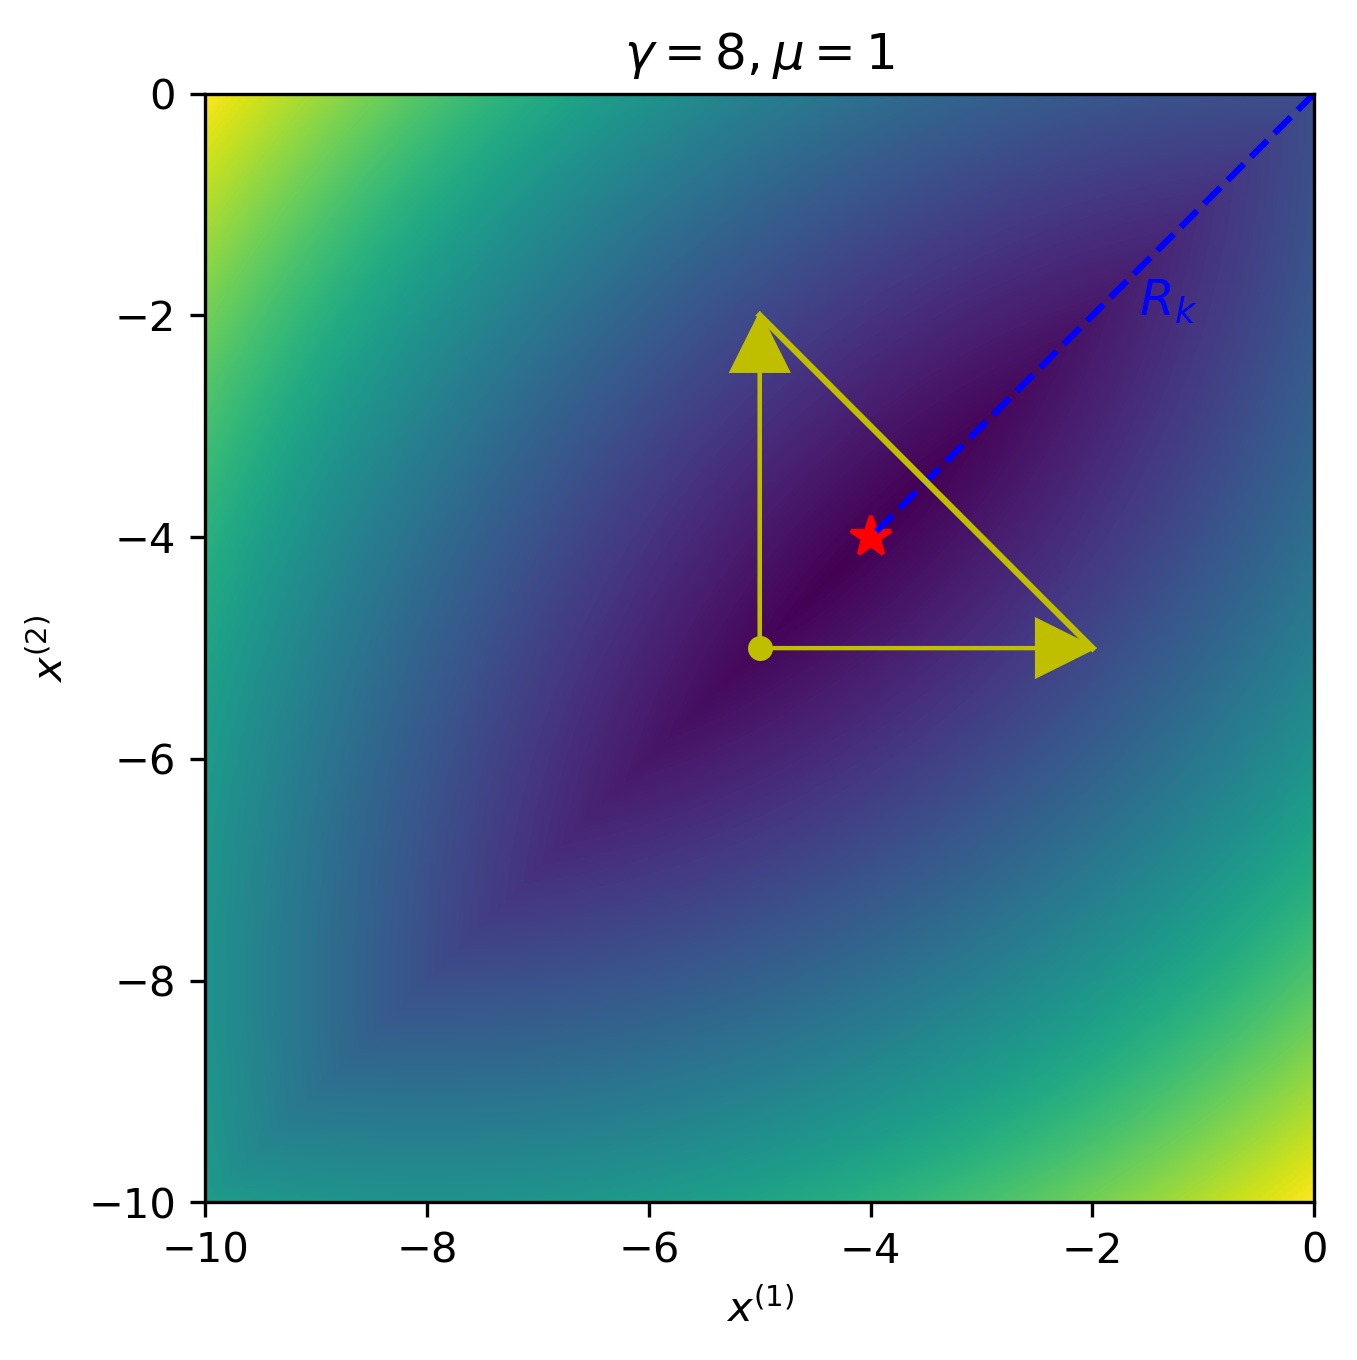
\includegraphics[width=\columnwidth]{fkImshow.png}
\end{figure}

\section*{3.2.2}

\begin{figure}[H]
    \centering
    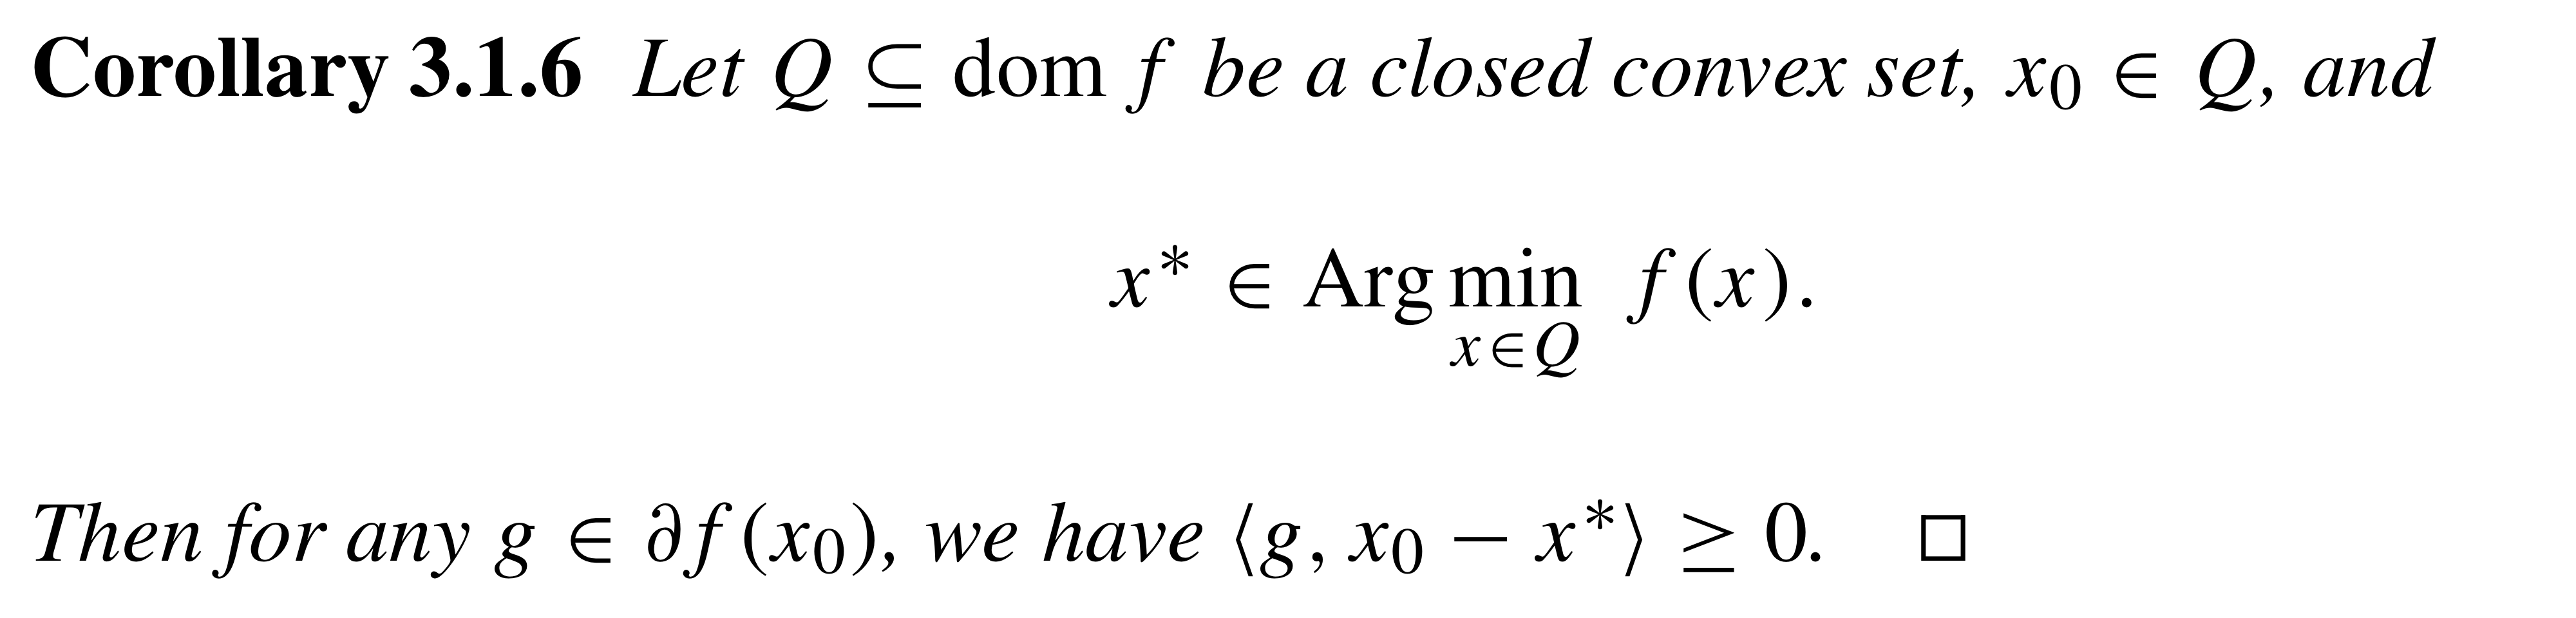
\includegraphics[width=\columnwidth]{col316.png}
    \caption{\red{p.199: ``We have justified this property in Corollary 3.1.6.''}}
\end{figure}

\section*{3.2.3}

\begin{figure}[H]
    \centering
    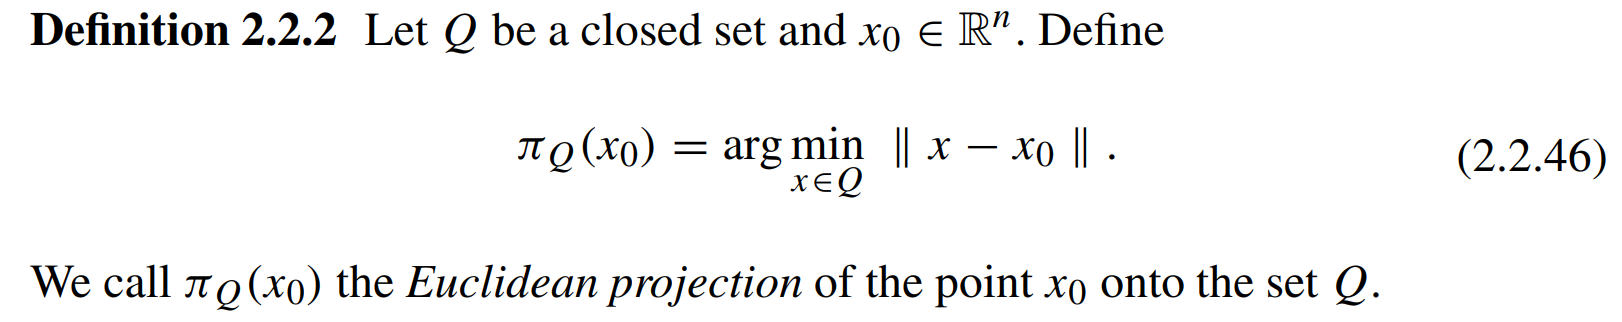
\includegraphics[width=\columnwidth]{def222.png}
    \caption{\red{p.202: ``$\pi_Q$''}}
\end{figure}

\begin{figure}[H]
    \centering
    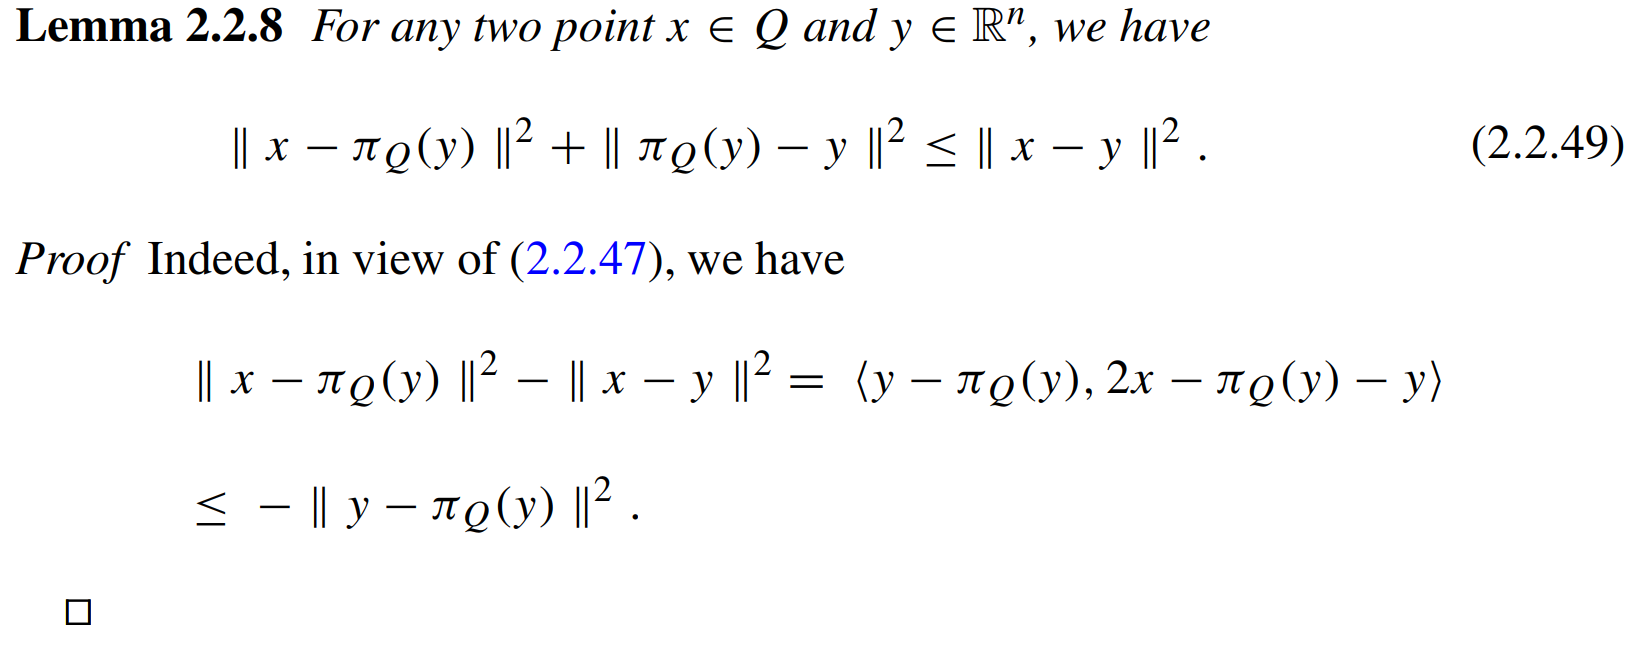
\includegraphics[width=\columnwidth]{lem228.png}
    \caption{\red{p.202: ``Then, in view of Lemma 2.2.8,''}}
\end{figure}

\begin{figure}[H]
    \centering
    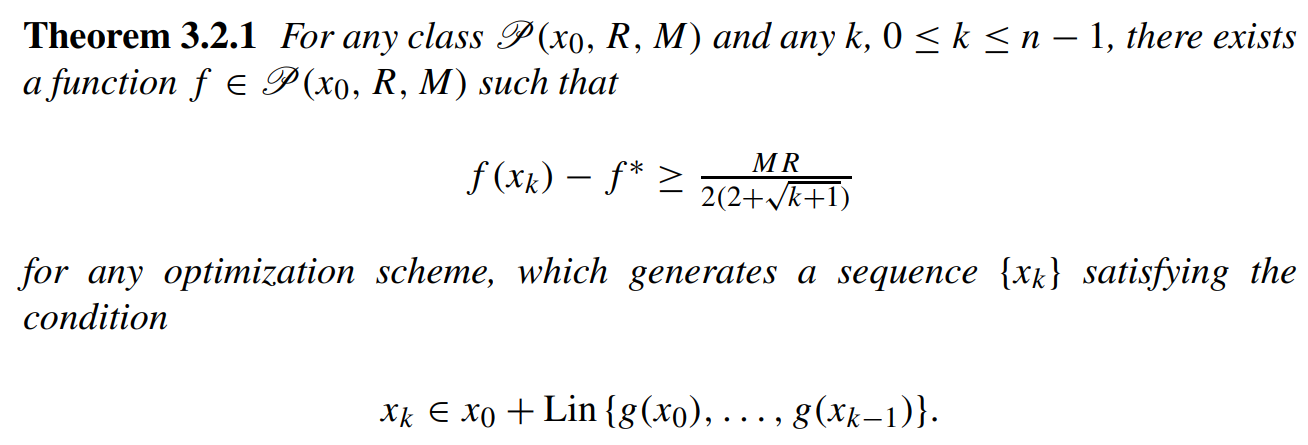
\includegraphics[width=\columnwidth]{thm321.png}
    \caption{\red{p.204: ``with the lower bound of Theorem 3.2.1''}}
\end{figure}


\section*{3.2.4}

\begin{figure}[H]
    \centering
    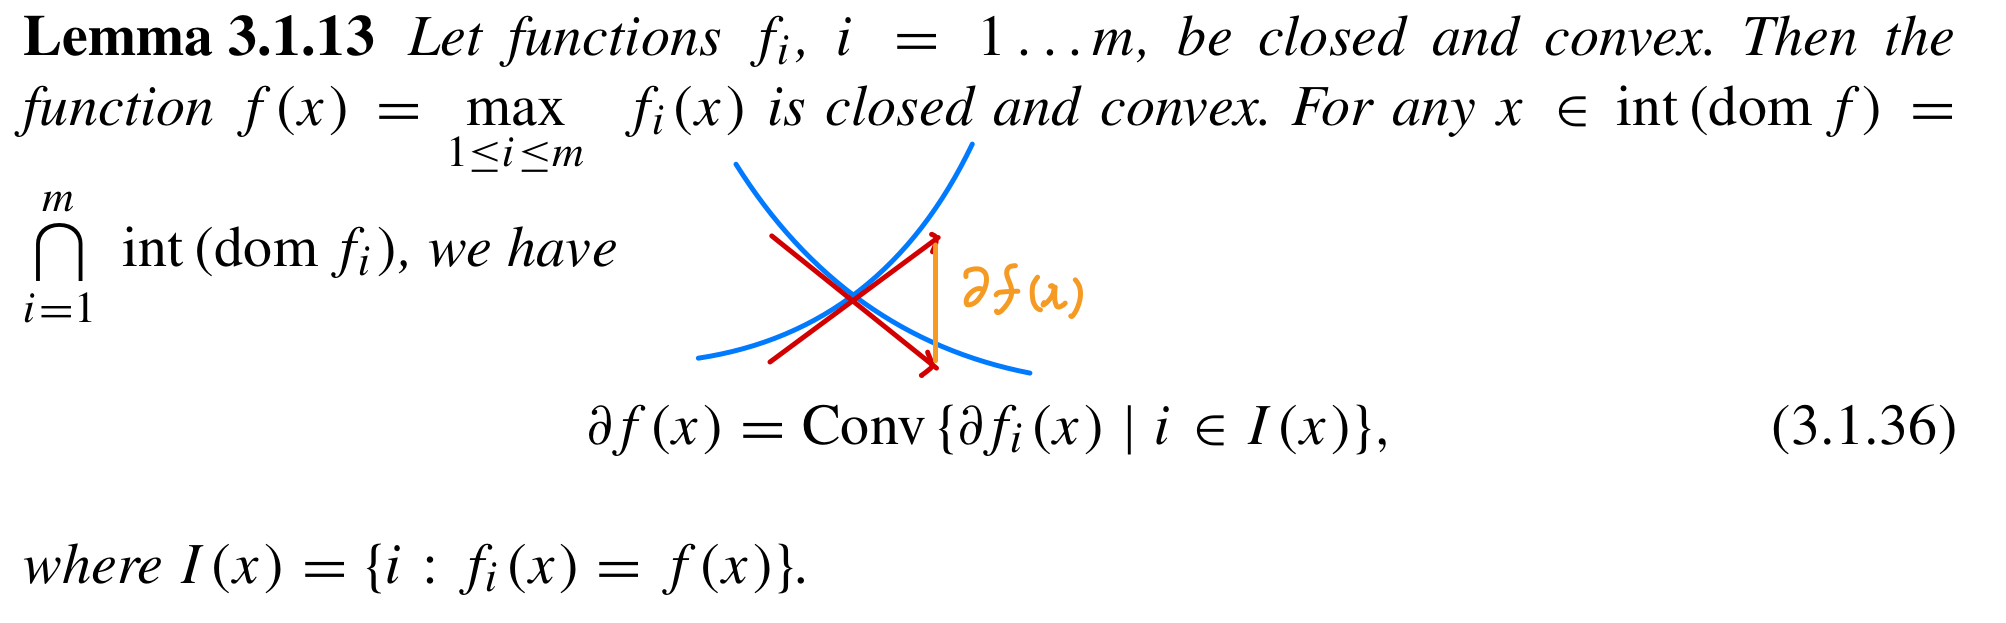
\includegraphics[width=\columnwidth]{lem3113.png}
    \caption{\red{p.205: ``we can do so for the functions $f_j$ (see Lemma 3.1.13)''}}
\end{figure}

\begin{figure}[H]
    \centering
    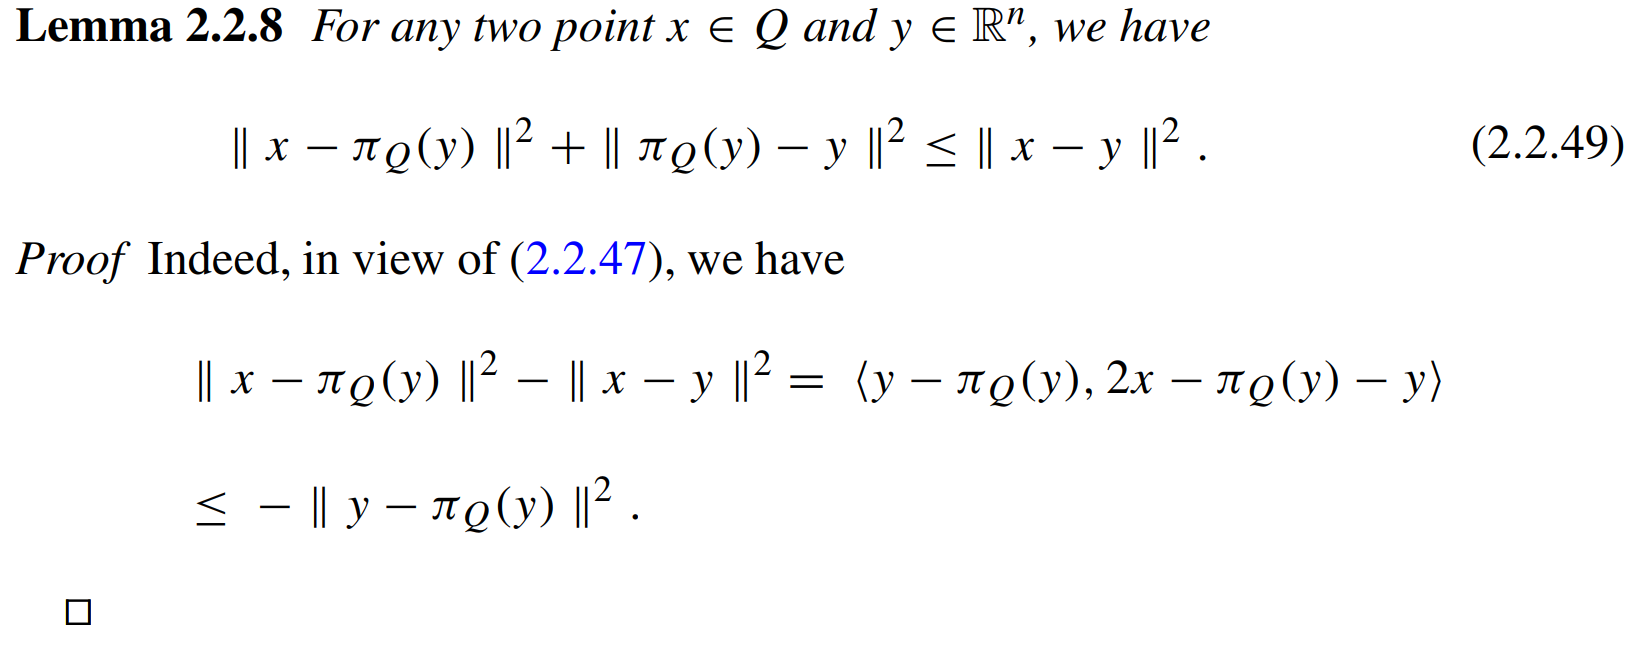
\includegraphics[width=\columnwidth]{lem228.png}
    \caption{\red{p.206: ``(2.2.49)''}}
\end{figure}

\begin{figure}[H]
    \centering
    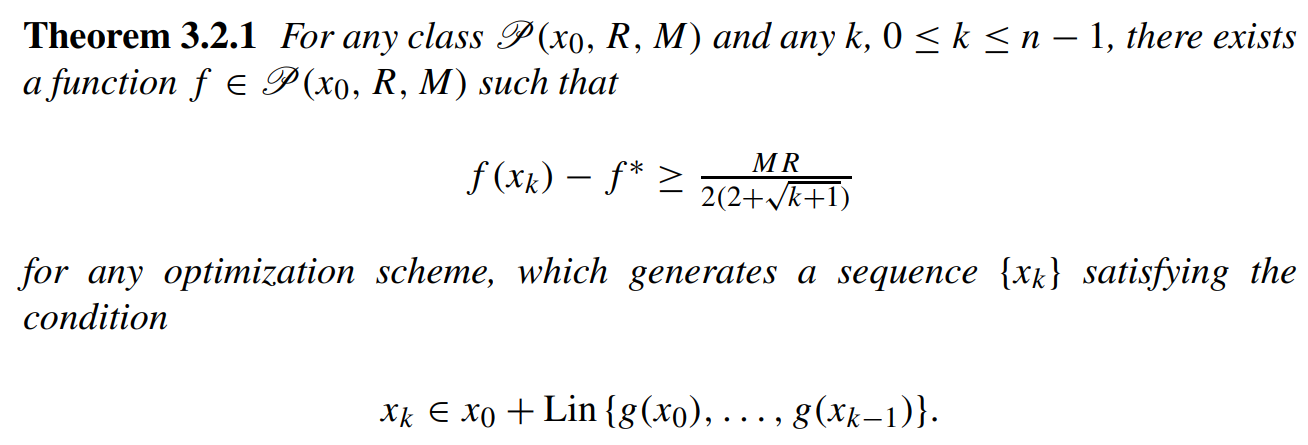
\includegraphics[width=\columnwidth]{thm321.png}
    \caption{\red{p.206: ``with the result of Theorem 3.2.1''}}
\end{figure}

\end{document}
